
%  PLEASE DO NOT REMOVE OR CHANGE THIS BLOCK
%  ===========================================================
%
%  A LaTeX Template for Typesetting Theses in Persian
%  By: Hamid Zarrabi-Zadeh
%  Source: https://github.com/zarrabi/thesis-template
%
%  License: Creative Commons Attribution 4.0
%  https://creativecommons.org/licenses/by/4.0/
%
%  Contributors: Ehsan Emamjomeh-Zadeh and Omid Gheibi
%  See the full list of contributors at GitHub.
%
%  ===========================================================


\documentclass[oneside,a4paper,12pt]{book}


% -------------------------------------------------------
%  Common Styles and Formattings
% -------------------------------------------------------


\usepackage{amssymb,amsmath}
\usepackage[colorlinks,linkcolor=blue,citecolor=blue]{hyperref}
\usepackage[usenames,dvipsnames]{pstricks}
\usepackage{graphicx,subfigure,wrapfig}
\usepackage{geometry}
\usepackage[mathscr]{euscript}
\usepackage{multicol}
\usepackage{multirow}
\usepackage[figureposition=bottom,tableposition=top,font={small,bf},labelfont=bf]{caption}

\usepackage{algorithmicx,algorithm}

\usepackage[localise=on,extrafootnotefeatures]{xepersian}
\usepackage[noend]{algpseudocode}


%------------------------ Algorithm ------------------------------------

\newenvironment{الگوریتم}[1]
	{\bigskip\bigskip\begin{algorithm}\caption{#1} \label{الگوریتم: #1}\vspace{0.5em}\begin{algorithmic}[1]}
	{\end{algorithmic}\vspace{0.5em}\end{algorithm}\bigskip}
	

\renewcommand{\algorithmicfor}{{به ازای}}
\renewcommand{\algorithmicwhile}{{تا وقتی}}
\renewcommand{\algorithmicdo}{\hspace{-.2em}:}
\renewcommand{\algorithmicif}{{اگر}}
\renewcommand{\algorithmicthen}{\hspace{-.2em}:}
\renewcommand{\algorithmicelse}{{در غیر این صورت:}}
%\renewcommand{\algorithmicelsif}{{در غیر این صورت اگر: }}
\renewcommand{\algorithmicreturn}{{برگردان}}
\renewcommand{\algorithmiccomment}[1]{$\triangleleft$ \emph{#1}}
\renewcommand{\algorithmicrequire}{\textbf{ورودی:}}
\renewcommand{\algorithmicensure}{\textbf{خروجی:}}

\newcommand{\اگر}{\If}
\newcommand{\وگرنه}{\Else}
\newcommand{\وگر}{\ElsIf}
\newcommand{\پایان‌اگر}{\EndIf}
\newcommand{\به‌ازای}{\For}
\newcommand{\پایان‌به‌ازای}{\EndFor}
\newcommand{\تاوقتی}{\While}
\newcommand{\پایان‌تاوقتی}{\EndWhile}
\newcommand{\دستور}{\State}
\newcommand{\دستورک}{\Statex}
\newcommand{\توضیحات}{\Comment}
\newcommand{\برگردان}{\Return}
\renewcommand{\ورودی}{\Require}
\newcommand{\خروجی}{\Ensure}



% -------------------- Page Layout --------------------


%\newgeometry{top=3cm,right=3cm,left=2.5cm,bottom=3cm,footskip=1.25cm}
\newgeometry{margin=1in,bottom=1.1in,footskip=.4in}

\renewcommand{\baselinestretch}{1.4}
\linespread{1.6}
\setlength{\parskip}{0.45em}

%\fancyhf{}
%\rhead{\leftmark}
%\lhead{\thepage}

\sloppy


% -------------------- Default Font --------------------

\settextfont[
Scale=1.09,
Extension=.ttf, 
Path=styles/fonts/,
BoldFont=XB NiloofarBd,
ItalicFont=XB NiloofarIt,
BoldItalicFont=XB NiloofarBdIt
]{XB Niloofar}

\setdigitfont[
Scale=1.09,
Extension=.ttf, 
Path=styles/fonts/,
BoldFont=XB NiloofarBd,
ItalicFont=XB NiloofarIt,
BoldItalicFont=XB NiloofarBdIt
]{XB Niloofar}


% -------------------- Sharif Font --------------------

\newcommand{\shariffont}{
\settextfont[
Scale=1.4,
Extension=.ttf, 
Path=styles/fonts/,
BoldFont=Sharif1.3-SemiBold,
]{Sharif1.3-Regular}

\setdigitfont[
Scale=1.4,
Extension=.ttf, 
Path=styles/fonts/,
BoldFont=Sharif1.3-SemiBold,
]{Sharif1.3-Regular}
}

% -------------------- Styles --------------------


\SepMark{-}
\renewcommand{\labelitemi}{$\small\bullet$}



% -------------------- Environments --------------------


\newtheorem{قضیه}{قضیه‌ی}[chapter]
\newtheorem{لم}[قضیه]{لم}
\newtheorem{ادعا}[قضیه]{ادعای}
\newtheorem{مشاهده}[قضیه]{مشاهده‌ی}
\newtheorem{نتیجه}[قضیه]{نتیجه‌ی}
\newtheorem{مسئله}{مسئله‌ی}[chapter]
\newtheorem{تعریف}{تعریف}[chapter]
\newtheorem{مثال}{مثال}[chapter]


\newenvironment{اثبات}
	{\begin{trivlist}\item[\hskip\labelsep{\em اثبات.}]}
	{\leavevmode\unskip\nobreak\quad\hspace*{\fill}{\ensuremath{{\square}}}\end{trivlist}}

\newenvironment{alg}[2]
	{\begin{latin}\settextfont[Scale=1.0]{Times New Roman}
	\begin{algorithm}[t]\caption{#1}\label{algo:#2}\vspace{0.2em}\begin{algorithmic}[1]}
	{\end{algorithmic}\vspace{0.2em}\end{algorithm}\end{latin}}


% -------------------- Titles --------------------


\renewcommand{\listfigurename}{فهرست شکل‌ها}
\renewcommand{\listtablename}{فهرست جدول‌ها}
\renewcommand{\bibname}{\rl{{مراجع}\hfill}} 


% -------------------- Commands --------------------


\newcommand{\IN}{\ensuremath{\mathbb{N}}} 
\newcommand{\IZ}{\ensuremath{\mathbb{Z}}} 
\newcommand{\IQ}{\ensuremath{\mathbb{Q}}} 
\newcommand{\IR}{\ensuremath{\mathbb{R}}} 
\newcommand{\IC}{\ensuremath{\mathbb{C}}} 

\newcommand{\set}[1]{\left\{ #1 \right\}}
\newcommand{\seq}[1]{\left< #1 \right>}
\newcommand{\ceil}[1]{\left\lceil{#1}\right\rceil}
\newcommand{\floor}[1]{\left\lfloor{#1}\right\rfloor}
\newcommand{\card}[1]{\left|{#1}\right|}
\newcommand{\setcomp}[1]{\overline{#1}}
\newcommand{\provided}{\,:\,}
\newcommand{\divs}{\mid}
\newcommand{\ndivs}{\nmid}
\newcommand{\iequiv}[1]{\,\overset{#1}{\equiv}\,}
\newcommand{\imod}[1]{\allowbreak\mkern5mu(#1\,\,\text{پیمانه‌ی})}

\newcommand{\poly}{\mathop{\mathrm{poly}}}
\newcommand{\polylog}{\mathop{\mathrm{polylog}}}
\newcommand{\eps}{\varepsilon}

\newcommand{\lee}{\leqslant}
\newcommand{\gee}{\geqslant}
\renewcommand{\leq}{\lee}
\renewcommand{\le}{\lee}
\renewcommand{\geq}{\gee}
\renewcommand{\ge}{\gee}

\newcommand{\مهم}[1]{\textbf{#1}}
\renewcommand{\برچسب}{\label}

\newcommand{\REM}[1]{}
\renewcommand{\حذف}{\REM}
\newcommand{\لر}{\lr}
\newcommand{\کد}[1]{\lr{\tt #1}}
\newcommand{\پاورقی}[1]{\footnote{\lr{#1}}}



% -------------------- Dictionary --------------------


\newcommand{\dicalphabet}[1]{
\begin{minipage}{\columnwidth}
	\centerline{\noindent\textbf{\large #1 }}
	\vspace{.5em}
\end{minipage}
\nopagebreak[4]
}

\newcommand{\dic}[2]{\noindent  #2 \dotfill  \lr{#1} \\ }


% ------------------------------ Images and Figures --------------------------

\graphicspath{{figs/}}
\setlength{\intextsep}{0pt}  % for float boxes
\renewcommand{\psscalebox}[1]{}  % for LaTeX Draw

\newcommand{\floatbox}[2]
	{\begin{wrapfigure}{l}{#1}
	\centering #2 \end{wrapfigure}}

\newcommand{\centerfig}[2]
	{\centering\scalebox{#2}{\input{figs/#1}}}

\newcommand{\fig}[3]
	{\floatbox{#3}{\centerfig{#1}{#2}}}

\newcommand{\centerimg}[2]
	{\vspace{1em}\begin{center}\includegraphics[width=#2]{figs/#1}\end{center}\vspace{-1.5em}}

\NewDocumentCommand{\img}{m m o}
	{\begin{wrapfigure}{l}{\IfValueTF{#3}{#3}{#2}}
	\centering\includegraphics[width=#2]{figs/#1}\end{wrapfigure}}




% -------------------------------------------------------
%  Custom Definitions
% -------------------------------------------------------


\newcommand{\OPT}{\ensuremath{\mathop{\mathrm{OPT}}}}
\newcommand{\APX}{\ensuremath{\mathop{\mathrm{APX}}}}
\newcommand{\ALG}{\ensuremath{\mathop{\mathrm{ALG}}}}



\begin{document}


% -------------------- Font Settings --------------------

%\shariffont  % برای استفاده از فونت شریف این خط را فعال کنید


% -------------------- Front Pages --------------------


% -------------------------------------------------------
%  Thesis Information
% -------------------------------------------------------

\newcommand{\ThesisType}
{پایان‌نامه}  % پایان‌نامه / رساله
\newcommand{\ThesisDegree}
{کارشناسی}  % کارشناسی / کارشناسی ارشد / دکتری
\newcommand{\ThesisMajor}
{مهندسی کامپیوتر}  % نام رشته / گرایش
\newcommand{\ThesisTitle}
{قالب استاندارد برای نگارش پایان‌نامه‌ها}  % عنوان پایان‌نامه / رساله
\newcommand{\ThesisAuthor}
{نام دانشجو}  % نام نویسنده
\newcommand{\ThesisSupervisor}
{استاد راهنمای پروژه}  % نام استاد راهنما
\newcommand{\ThesisAdvisor}
{استاد مشاور}  
\newcommand{\ThesisExaminer}
{استاد ممتحن}
\newcommand{\ThesisDate}
{شهریور ۱۴۰۳}
\newcommand{\ThesisDepartment}
{دانشکده مهندسی کامپیوتر}
\newcommand{\ThesisUniversity}
{دانشگاه صنعتی شریف}

% -------------------------------------------------------
%  English Information
% -------------------------------------------------------

\newcommand{\EnglishThesisDegree}{B.Sc.}

\newcommand{\EnglishThesisTitle}{A Standard Template for Typesetting Theses in Persian}

\newcommand{\EnglishThesisAuthor}{The Author}

\newcommand{\EnglishThesisSupervisor}{Dr. Supervisor}

\newcommand{\EnglishThesisDate}{September 2024}

\newcommand{\EnglishThesisDepartment}{Department of Computer Engineering}

\newcommand{\EnglishThesisUniversity}{Sharif University of Technology}

\pagestyle{empty}

% -------------------------------------------------------
%  Title Page
% -------------------------------------------------------


% راهنمایی: اطلاعات پایان‌نامه را در فایل front/info.tex ویرایش کنید.

\begin{center}


\includegraphics[scale=0.25]{front/template/images/logo}

\vspace{-0.2cm}
\ThesisUniversity \\[-0.3em]
\ThesisDepartment

\begin{large}
\vspace{0.5cm}

\ThesisType \ \ThesisDegree \\[-0.3em]
\ThesisMajor

\end{large}

\vspace{2cm}

{\LARGE\textbf{\ThesisTitle}}

\vspace{2.5cm}

{نگارش}\\[.5em]
{\large\textbf{\ThesisAuthor}}

\vspace{0.7cm}

{استاد راهنما}\\[.5em]
{\large\textbf{\ThesisSupervisor}}

\vspace{1.3cm}

\ThesisDate

\end{center}



% info: برای درج هر یک از صفحات زیر، خط مربوطه را فعال کنید

%
% -------------------------------------------------------
%  Besmellah Page
% -------------------------------------------------------

\begin{center}


\includegraphics[width=0.45\textwidth]{front/template/images/besmellah}

\end{center}
  % صفحه بسم الله
%
% -------------------------------------------------------
%  Signatures Page
% -------------------------------------------------------

\begin{large}
\setlength{\parindent}{0pt}
\begin{center}

%{\large\bf تصویب‌نامه}\\
\vspace{1em}

{\normalsize\bf به نام خدا}

{\normalsize
\ThesisUniversity\\[-0.1cm]
\ThesisDepartment}

\vspace{2.5em}
\textbf{\large\ThesisType \ \ThesisDegree}

\vspace{0.5em}
این \ThesisType\ به عنوان تحقق بخشی از شرایط دریافت درجه \ThesisDegree\ است.
\end{center}

\vspace{1.5em}

{\large \textbf{عنوان}: \ThesisTitle}

\vspace{.3em}

{\large \textbf{نگارش}: \ThesisAuthor}

\vspace{1cm}

\textbf{کمیته ممتحنین}

\vspace{1em}
\begin{tabular}{p{7cm}r}
استاد راهنما: \ThesisSupervisor & امضاء: \\[1.5em]
استاد مشاور: \ThesisAdvisor & امضاء: \\[1.5em]
استاد مدعو: \ThesisExaminer & امضاء: \\[2em]
& تاریخ:
\end{tabular}

\end{large}

  % صفحه تصویب‌نامه
%
% -------------------------------------------------------
%  Declaration Page
% -------------------------------------------------------

{\parindent0pt

\begin{center}
{\large\bf اظهارنامه}

{\small(اصالت متن و محتوای \ThesisType{} \ThesisDegree)}
\end{center}
\vspace{-6em}

\includegraphics[scale=0.18]{front/template/images/logo}
\vspace{1em}

\textbf{عنوان ‌\ThesisType}: \ThesisTitle

\vspace{.1em}
\begin{multicols}{2}
	{\مهم{استاد راهنما}: \ThesisSupervisor}
	
	{\مهم{استاد مشاور}: \ThesisAdvisor}
\end{multicols}

\vspace{0.2em}
\کوچک
این‌جانب {\ThesisAuthor} اظهار می‌دارم:
\شروع{شمارش}
\فقره متن و نتایج علمی ارائه شده در این \ThesisType{} اصیل بوده و زیرنظر استادان نام‌برده ‌شده در بالا تهیه شده است.
\فقره متن \ThesisType{} به این صورت در هیچ جای دیگری منتشر نشده است.
\فقره متن و نتایج مندرج در این \ThesisType، حاصل تحقیقات این‌جانب به عنوان دانشجوی \ThesisDegree{} دانشگاه صنعتی شریف است.
\فقره کلیه مطالبی که از منابع دیگر در این \ThesisType{} مورد استفاده قرار گرفته، با ذکر مرجع مشخص شده است.
\پایان{شمارش}

\begin{multicols}{2}
\ \\
\ \\
\ \\

نگارنده: \ThesisAuthor\\
تاریخ: \\
امضاء: \\
\end{multicols}

نتایج تحقیقات مندرج در این \ThesisType{} و دستاوردهای مادی و معنوی ناشی از آن (شامل فرمول‌ها، توابع کتابخانه‌ای، نرم‌افزارها، سخت‌افزارها و مواردی که قابلیت ثبت اختراع دارد) متعلق به دانشگاه صنعتی شریف است. هیچ شخصیت حقیقی یا حقوقی بدون کسب اجازه از دانشگاه صنعتی شریف حق فروش و ادعای مالکیت مادی یا معنوی بر آن یا ثبت اختراع از آن را ندارد. همچنین، کلیه حقوق مربوط به چاپ، تکثیر، نسخه‌برداری، ترجمه، اقتباس و نظائر آن در محیط‌های مختلف اعم از الکترونیکی، مجازی یا فیزیکی برای دانشگاه صنعتی شریف محفوظ است. نقل مطلب با ذکر ماخذ بلامانع است.


\begin{multicols}{2}
استاد راهنما: \ThesisSupervisor \\
تاریخ: \\
امضاء: \\

نگارنده: \ThesisAuthor\\
تاریخ: \\
امضاء: \\
\end{multicols}
}

  % صفحه اظهارنامه

\pagestyle{plain}
\pagenumbering{tartibi}

%
% -------------------------------------------------------
%  Acknowledgments
% -------------------------------------------------------


\begin{center}
\مهم{سپاس}
\end{center}

از استاد بزرگوارم که با کمک‌ها و راهنمایی‌های بی‌دریغشان، مرا
در به سرانجام رساندن این پایان‌نامه یاری داده‌اند، تشکر و قدردانی می‌کنم.
همچنین از همکاران عزیزی که با راهنمایی‌های خود در بهبود نگارش این نوشتار
سهیم بوده‌اند، صمیمانه سپاسگزارم.

  % صفحه سپاس

% -------------------------------------------------------
%  Abstract
% -------------------------------------------------------



% -------------------------------------------------------
%  Abstract
% -------------------------------------------------------


\شروع{وسط‌چین}
\مهم{چکیده}
\پایان{وسط‌چین}
\بدون‌تورفتگی

در این پروژه بنا داریم تا در ابتدا با محیط برنامه نویسی EFI آشنا شویم به همین سبب کد Hello World با استفاده از EFI می‌نویسیم و گزارشی از آن ارائه می‌دهیم. در ادامه کمی در رابطه با آزمون حافظه، پیاده‌سازی آن و الگوریتم‌های آن تحقیق می‌کنیم. در آخر مقداری با Boot امن آشنا خواهیم شد و ...


کامل شه



% -------------------- Table of Contents --------------------

\tableofcontents \newpage
%\listoftables \newpage
\listoffigures \newpage


% -------------------- Chapters --------------------

\pagenumbering{arabic}


\فصل{نوشتن برنامه Hello World با EFI}

در این قسمت برای شروع کار یک برنامه‌ی Hello World می‌نویسیم.

\قسمت{آماده کردن محیط برنامه نویسی EFI}

برای این قسمت ما از \لر{edk2} استفاده کرده‌ایم که می‌توانید آن را در این \href{https://github.com/tianocore/edk2}{لینک} مشاهده کنید. این ابزار یک سری کتابخانه برای نوشتن و ساختن برنامه‌ها و درایورهای \لر{EFI} است.

\قسمت{تحلیل کد}

کد این قسمت در \لر{HelloWorld.c} نوشته شده است. تابع \لر{UefiMain} تابعی است که در شروع برنامه اجرا می‌شود. در خط اول توسط تابع \لر{Print} رشته مورد نظر را چاپ می‌کنیم و دقت می‌کنیم که در \لر{UEFI} باید از رشته‌های عریض (کاراکترهای ۲ بایتی) استفاده شود.

\قسمت{اجرای کد}
برای اجرای کد با استفاده از \لر{QEMU} و \لر{OVMF} یک محیط \لر{EFI} بالا می‌آوریم تا برنامه را در آن اجرا کنیم. این کار با دادن \لر{OVMF} به عنوان آپشن \لر{bios} به \لر{QEMU} به سادگی قابل انجام است. این اجرا در \رجوع{fig:helloworld1} قابل مشاهده است.
\begin{figure}
	\centering
	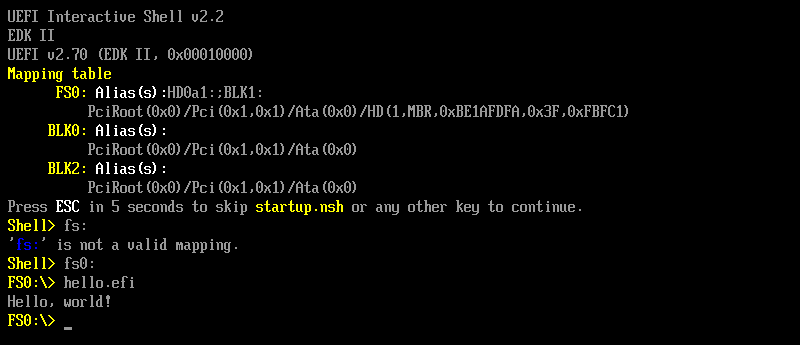
\includegraphics[width=0.7\linewidth]{figs/helloworld/helloworld1}
	\caption{اجرای برنامه‌ی \لر{hello.efi}}
	\label{fig:helloworld1}
\end{figure}


\فصل{آزمون حافظه}



\قسمت{آشنایی با آزمون حافظه}

آزمون حافظه به فرایند تست کردن و تایید کردن کارکرد، درستی و کارایی حافظه سیستم می‌گویند که می‌تواند شامل حافظه فیزیکی و یا حافظه مجازی شود. از این آزمون‌ها برای پیدا کردن خطاها، اعتبارسنجی حافظه فیزیکی، بررسی کارایی و تخصیص دادن حافظه استفاده 
کرد. آزمون حافظه‌ای که ما استفاده می‌کنیم از نوع Power-On Self-Test(POST) است یعنی 
هنگام Boot کامپیوتر، BIOS یک تست ساده را اجرا کند تا از کارایی حافظه مطمئن شود.

\قسمت{انواع آزمون‌های حافظه}

\زیرقسمت{Pattern Testing}

در این روش یک الگویی از داده‌ها را در حافظه می‌نویسیم و در آخر آن بخشها را می‌خوانیم و یکی بودنشان را بررسی می‌کنیم.

\زیرقسمت{Stress Testing}

برای شبیه‌سازی دنیای واقعی حافظه را  با خواندن و نوشت نبه شدت لود می‌کنیم تا پایداری آن را در این شرایط بسنجیم.

\قسمت{پیاده‌سازی آزمون حافظه}

برای پیاده‌سازی آزمون حافظه در ابتدا با متغیر pattern که توان‌هایی از 2 است را در خانه‌هایی از حافظه می‌نویسیم و سپس مقادیر همان خانه‌ها را می‌خوانیم و یکی بودنشان را بررسی می‌کنیم این کلیت آزمون اول یعنی آزمون WalkingOnesTest می‌باشد.

در ادامه کد تستی برای حالت چندپردازه خواهیم داشت که در آن بنابر آیدی پردازه بررسی می‌کنیم که در صفحه مربوط به آن پردازه هستیم یا نه و سپس در هر خانه م نظر آدرس آن خانه را می‌نویسیم و در آخر دوباره همه‌ی این مقادیر را می‌خوانیم تا از صحت اطلاعات مطمئن شویم.



\فصل{نکات پیاده‌سازی}

\قسمت{یکپارچه‌سازی با \لر{Shell}}

در این قسمت ما با استفاده از کتابخانه \لر{ShellCEntryLib} تابع ورودی کد را مانند یک تابع ورودی عادی در \لر{C} کردیم. سپس با استفاده از دستور \لر{alias} در شل آن را مانند دستورات عادی کردیم. این کار دائمی است و بین دو بوت متوالی از بین نمی‌رود. همچنین با صدا زدن کد مانند \لر{memtest testname} می‌توان فقط یک تست خاص را اجرا کرد که در \رجوع{fig:impl1} قابل مشاهده است.

\قسمت{پیاده‌سازی چندهسته‌ای آزمون \لر{Identity}}

برای این کار ما از پروتکل \لر{MpService} در \لر{UEFI} استفاده کردیم. یک تابع کارگر ساختیم و سپس با استفاده از \لر{StartupAllAPs} آن را روی هسته‌های مختلف فراخوانی کردیم.

\begin{figure}
	\centering
	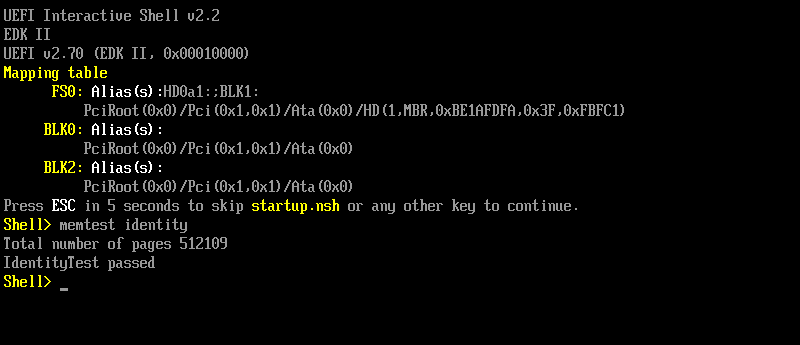
\includegraphics[width=0.7\linewidth]{figs/impl/impl1}
	\caption{صدا زدن برنامه و اجرای تست \لر{Identity}}
	\label{fig:impl1}
\end{figure}

\قسمت{پیاده‌سازی \لر{GUI}}

ما تلاش کردیم تا یک محیط گرافیکی ساده برای این برنامه ارائه دهیم اما به مشکل خوردیم. اصلی ترین مشکلی که داشتیم این بود که در حین آزمون نباید حافظه جدیدی اختصاص داده می‌شود، وگرنه ممکن بود آزمون ما با یک سامانه دیگر تداخل بخورد و آزمون و/یا روند اجرای یک تابع بیرونی به غلط انجام شوند. کتاب‌خانه‌هایی که اجزای گرافیکی را پیاده‌سازی کرده بودند ممکن بود با اجرا شدن از سیستم حافظه بگیرند و این باعث می‌شد که ما نتوانیم از آن‌ها وسط آزمون استفاده کنیم. به عبارتی دیگر برای پیاده‌سازی یک رابط گرافیکی باید کتاب‌خانه‌های مربوطه را در سطح پایین تغییر می‌دادیم که از حافظه‌های از قبل اختصاص داده شده استفاده کنند که به علت کمبود زمان موفق به انجام این مورد نشدیم.

\def\myfigure#1#2{ \شروع{شکل}[ht]
\centerimg{#1}{14cm}
\شرح{#2}
\پایان{شکل}
}

\def\lrtt#1{\lr{\tt #1}}

\فصل{بوت امن}

بوت امن (\lr{Secure Boot}) یکی از ویژگی‌های امنیتی سیستم‌های \lr{UEFI} است که هدف آن جلوگیری از اجرای
کدهای غیرمجاز در فرآیند بوت سیستم می‌باشد. در این فرآیند، تمام نرم‌افزارهای بوت باید دارای امضای
دیجیتال معتبر باشند. ابزار \lr{shim} یک واسط است که به کاربران امکان می‌دهد گواهی‌های سفارشی یا کلیدهای
اضافی را برای بوت امن اضافه کنند، به خصوص در سیستم‌های لینوکسی که ممکن است امضاهای استاندارد
مایکروسافت را نداشته باشند. این روش باعث حفظ امنیت در عین انعطاف‌پذیری می‌شود.

از آنجا که خروجی \lr{EFI} ما امضای رسمی مایکروسافت را ندارد، به \lr{shim} برای اجرای آن در محیط بوت امن نیاز داریم.

\قسمت{شبیه‌سازی}

برای شبیه‌سازی بوت امن از \lr{Virtualbox} استفاده می‌کنیم. در این محیط می‌توانیم \lr{EFI} و بوت امن را
مشابه ماشین واقعی تست کنیم.  یک سیستم عامل مجازی اوبونتو نصب می‌کنیم تا عملیات‌های مرتبط با راه‌اندازی
برنامه را در آن انجام دهیم.

\قسمت{آماده‌سازی برنامه}

باید به برنامه \lr{section} به نام \lr{sbat} اضافه کنیم. مهم است مقدار آن را \lr{shim} بشناسد و به
همین خاطر از بخش مشابهی در \lr{grub} استفاده می‌کنیم.

\myfigure{sec/01}{اضافه کردن \lr{sbat}}

\قسمت{آماده‌سازی بوت}

برنامه \lr{shim} به طور پیشفرض در اوبونتو نصب می‌شود. لازم است فایل‌های \lr{shim} و برنامه \lr{EFI} را
به پارتیشن \lr{ESP} منتقل می‌کنیم. اسم برنامه را به \lrtt{grubx64.efi} تغییر می‌دهیم. به صورت
پیشفرض \lr{shim} برنامه‌ای با این اسم را لود می‌کند.

\myfigure{sec/02}{کپی کردن \lr{shim} به \lr{ESP}}
\myfigure{sec/03}{اضافه کردن \lr{boot option}}

\قسمت{بوت با اثرانگشت برنامه}

یک راه برای بوت امن این است که اجازه دهیم \lr{shim} بوت شود و سپس اثرانگشت برنامه را به \lr{MokList}
اضافه کنیم. بعد از انجام این کار \lr{shim} برنامه را اجرا می‌کند و خطای \lrtt{0x1a Security
Violation} چاپ نمی‌شود.  مراحل اضافه کردن اثرانگشت \lr{hash} در ادامه نشان داده شده است.

\myfigure{sec/06}{صفحه \lr{Mok Management}}
\myfigure{sec/07}{وارد کردن امضای برنامه}
\myfigure{sec/08}{منوی انتخاب برنامه‌ها}

\قسمت{بوت با امضای برنامه}

راه دیگر برای بوت امن این است که یک کلید شخصی بسازیم و برنامه \lr{EFI} را با آن امضا کنیم. بعد از
امضا کردن و اجرای دوباره \lr{shim}، می‌توانیم فایل \lr{DER} امضا را به \lr{MokList} اضافه کنیم. مزیت
این روش این است که اگر برنامه بعدا تغییر کند فقط لازم است یک بار دیگر آن را امضا کنیم و دیگر طی کردن
مراحل \lr{enroll key} لازم نیست.

\myfigure{sec/04}{ساخت کلید}
\myfigure{sec/05}{امضای برنامه \lr{EFI}}

\قسمت{منابع}

\begin{latin}
\url{https://wiki.archlinux.org/title/Unified_Extensible_Firmware_Interface/Secure_Boot}

\url{https://www.funtoo.org/UEFI_Secure_Boot_and_SHIM}

\url{https://github.com/rhboot/shim/blob/main/SBAT.md}

\url{https://github.com/rhboot/shim/issues/376}
\end{latin}



% -------------- Bibliography & Dictionary ---------------

%
% -------------------------------------------------------
%  Bibliography
% -------------------------------------------------------

\clearpage
\phantomsection
\addcontentsline{toc}{chapter}{مراجع}

\begin{latin}
\baselineskip=.8\baselineskip
\bibliographystyle{./styles/packages/unsrtabbrv}

% Uncomment next line to include uncited references
% \nocite{*}

\bibliography{bibs/full,bibs/refs}
 
\end{latin}

%
\clearpage
\phantomsection
\addcontentsline{toc}{chapter}{واژه‌نامه}

\chapter*{واژه‌نامه}
\begin{multicols}{2}
\small

\dicalphabet{الف}
\dic{heuristic}{ابتکاری}
\dic{high dimensions}{ابعاد بالا}
\dic{bias}{اریب}
\dic{threshold}{آستانه}
\dic{pigeonhole principle}{اصل لانه‌ی کبوتری}
\dic{NP-Hard}{ان‌پی‌-سخت}
\dic{transition}{انتقال}

\dicalphabet{ب}
\dic{online}{برخط}
\dic{linear programming}{برنامه‌ریزی خطی}
\dic{optimum}{بهینه}
\dic{maximum}{بیشینه}

\dicalphabet{پ}
\dic{outlier}{پرت}
\dic{query}{پرسمان}
\dic{cover}{پوشش}
\dic{complexity}{پیچیدگی}

\dicalphabet{ت}
\dic{experimental}{تجربی}
\dic{density}{تراکم}
\dic{approximation}{تقریب}
\dic{partition}{تقسیم‌بندی}
\dic{mesh}{توری}
\dic{distributed}{توزیع‌شده}

\dicalphabet{ج}
\dic{separable}{جداپذیر}
\dic{black box}{جعبه سیاه}
\dic{data stream}{جویبار داده}

\dicalphabet{ح}
\dic{extreme}{حدی}
\dic{greedy}{حریصانه}

\dicalphabet{خ}
\dic{cluster}{خوشه}
\dic{linear}{خطی}

\dicalphabet{د}
\dic{data}{داده}
\dic{data mining}{داده‌کاوی}
\dic{outlier data}{داده‌ی پرت}
\dic{doubling}{دوبرابرسازی}
\dic{binary}{دودویی}

\dicalphabet{ر}
\dic{vertex}{رأس}
\dic{formal}{رسمی}

\dicalphabet{ز}
\dic{sublinear}{زیرخطی}

\dicalphabet{س}
\dic{amortized}{سرشکن}
\dic{hierarchichal}{سلسه‌مراتبی}

\dicalphabet{ش}
\dic{pseudocode}{شبه کد}
\dic{object}{شیء}

\dicalphabet{ص}
\dic{satisfiability}{صدق‌پذیری}

\dicalphabet{غ}
\dic{dominate}{غلبه}

\dicalphabet{ف}
\dic{distance}{فاصله}
\dic{space}{فضا}

\dicalphabet{ق}
\dic{deterministic}{قطعی}

\dicalphabet{ک}
\dic{efficient}{کارا}
\dic{candidate}{کاندیدا}
\dic{minimum}{کمینه}

%\dicalphabet{گ}
%\dic{pass}{گذر}

\dicalphabet{م}
\dic{set}{مجموعه}
\dic{coreset}{مجموعه هسته}
\dic{planar}{مسطح}
\dic{parallelization}{موازی‌سازی}
\dic{buffer}{میان‌گیر}

\dicalphabet{ن}
\dic{inversion}{نابه‌جایی}
\dic{invariant}{ناوردا}
\dic{center point}{نقطه‌ی مرکزی}
\dic{half space}{نیم‌فضا}

\dicalphabet{هـ}
\dic{price of anarchy (POA)}{هزینه‌ی آشوب}

\dicalphabet{ی}
\dic{edge}{یال}

\end{multicols}




% -------------------- Appendices --------------------

%\begin{appendix}
%
\فصل{مطالب تکمیلی}

پیوست‌های خود را در صورت وجود می‌توانید در این قسمت قرار دهید. 



%\end{appendix}


% -------------------- English Pages --------------------

%\newgeometry{left=3cm,right=2.5cm}

%\pagestyle{empty}
%
% -------------------------------------------------------
%  English Abstract
% -------------------------------------------------------

\begin{latin}

\begin{center}
\textbf{Abstract}
\end{center}
\baselineskip=.8\baselineskip

We present a standard template for typesetting theses in Persian. 
The template is based on the \XePersian\ package for the \LaTeX\ typesetting system.
This write-up shows a sample usage of this template.


\bigskip\noindent\textbf{Keywords}:
Thesis, Typesetting, Template, \XePersian\

\end{latin}

%
% -------------------------------------------------------
%  English Title Page
% -------------------------------------------------------

\begin{center}

\begin{latin}


\includegraphics[scale=0.25]{front/template/images/logo}

\EnglishThesisUniversity \\
\EnglishThesisDepartment

\begin{large}
\vspace{0.7cm}
\EnglishThesisDegree{} Thesis


\vspace{1.5cm}

{\Large\textbf\EnglishThesisTitle}

\vspace{1.5cm}

{\normalsize By:}\\
\textbf{\EnglishThesisAuthor}

\vspace{1cm}

{\normalsize Supervisor:}\\ 
\textbf{\EnglishThesisSupervisor}

\end{large}

\vspace{1.5cm}
\EnglishThesisDate

\end{latin}

\end{center}



% -------------------- The End! --------------------

\end{document}

